\documentclass[a4paper, 11pt]{article}
\usepackage{comment} % enables the use of multi-line comments (\ifx \fi) 
\usepackage{lipsum} %This package just generates Lorem Ipsum filler text. 
\usepackage{fullpage} % changes the margin
\usepackage{graphicx}
\usepackage{epsfig}

\begin{document}
%Header-Make sure you update this information!!!!
\noindent
\large\textbf{Lab 1 Report} \hfill \textbf{Abhishek Srivastava} \\
\normalsize CS260-001: Computer Security \hfill Student Id: 861307778 \\
\hrule

\section*{Problem 1: Code Injection}
Construct an exploit input that can inject a shell code to be executed in the vulnerable program.

\section*{Solution 1}
As per the system architecture buffer overflow will overwrite the \textbf{old ebp address}, \textbf{return address of} \emph{IsPasswordOkay} function and its offsets from the location of string input in the program going upward. To execute the instructions in \textbf{codeinjection.bin} we have to put correct value in the return address location.\\

To find out the location to be overwritten I found out the ebp address while in the /emph{IsPasswordOkay} function. I put break point at IsPasswordOkay function using gdb and check the registers values using command \{\textbf{i r}\}.\\

From Figure 1 we can see that while in the \emph{IsPasswordOkay} function (Breakpoint 1) the ebp address is \textbf{0xffffce28}, so above it is return address location and above it is offsets location and above that is the locations of buffer overwritten data. So I added 30 bytes which gave me address \textbf{0xffffce46}. This is the address we need to replace in the return function address so the values above it can be read and executed.\\

Also to prevent the segmentation error I wrote the correct old ebp address which was overwritten by the buffer overflow. To found out the old ebp address, I put break point on main() and then checked the register values. From figure one we can see that old epb address is \textbf{0xffffce48}. This is the value to be written in the old ebp address location so that segmentation error will not occur.\\

So after the 20 bytes in the binary file we can insert old ebp address which is \textbf{0xffffce48}, it should be written in little endian method (48,CE,FF,FF) and then next 4 bytes the return address which is \textbf{0xffffce46} can be written as (46,CE,FF,FF). Figure 2 shows the edited binary file. This will be the input file while executing the program.\\

Figure 3 shows the result of running the buffer overflow exploit input for the program entered through edited binary file. The program is successfully executed and we can see the output with no segmentation error and program exited normally.

\begin{figure}
	\centering
	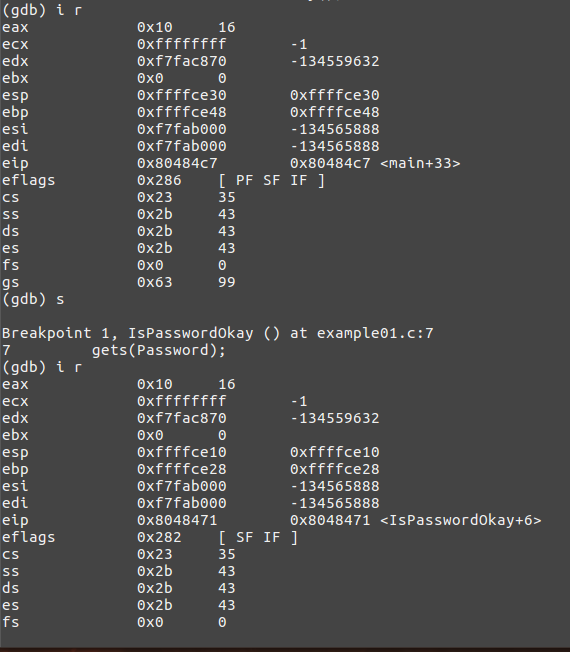
\epsfig{file=prob_1_part_1.png, height=8in, width=6.5in}
	\caption{Register Values before and after calling IsPasswordOkay function.}
\end{figure}
\begin{figure}
	\centering
	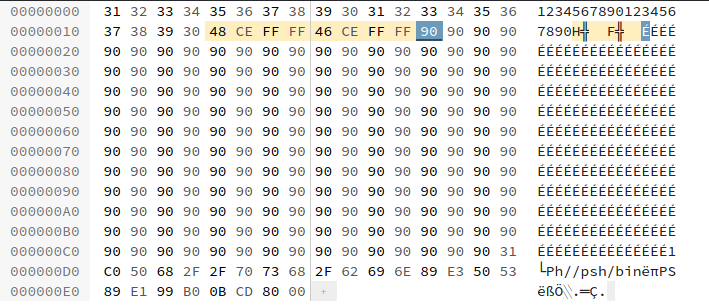
\epsfig{file=prob_1_part_2.png, height=3in, width=7in}
	\caption{Binary files with edited values.}
\end{figure}
\begin{figure}
	\centering
	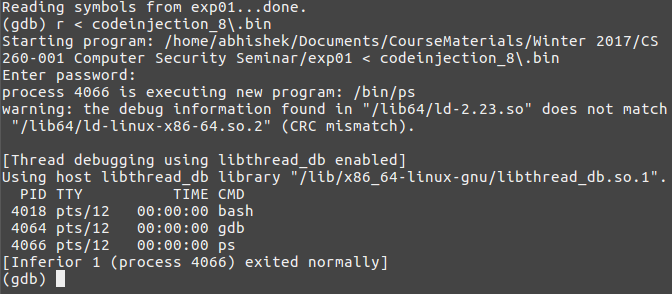
\epsfig{file=prob_1_part_3.png, height=4in, width=7in}
	\caption{Output of buffer overflow exploit.}
\end{figure}
\newpage
\section*{Problem 2: Return to libc}
Construct an expoit input that takes advantage of the existing “system” library call in libc to achieve the same goal as in the first task. That is, we want to run “ps” command, without injecting any code into the stack of the vulnerable program.
\section*{Solution 2}
Solution 2 is also similar to the Solution 1. The main things we have to identify for this problem are:
\begin{itemize}
	\item System Address : \textbf{p system} command gives the system address.
	\item Exit Address: \textbf{p exit} command gives the system address.
	\item Return Address of the inputs: This we have to calculate.
\end{itemize}

Figure 4 shows the address of system and exit. We are giving address of exit for a smooth termination of system call.\\

Similar to Problem 1 from Figure 1 we know that the ebp address is \textbf{0xffffce28}, so above it is return address location and above it is offsets location and above that is the locations of buffer overwritten data. So I added 12 bytes to skip the addresses which is to be overwritten with system address and exit address which gave me the address \textbf{0xffffce3a}. This is the address we need to replace in the next 4 bytes so the values above it can be read and passed into system call and then executed.\\

Also to prevent the segmentation error like in problem 1 I wrote the correct old ebp address which we know from previous problem is \textbf{0xffffce48}.\\

So after the 20 bytes in the binary file we can insert the old ebp address which is \textbf{0xffffce48}, it should be written in little endian method (48,CE,FF,FF), then next 4 bytes the system address which is \textbf{0xf7e33da0} can be written as (A0,3D,E3,F7), next for 4 bytes the address of exit which is \textbf{0xf7e279d0} can be written as (D0,79,E2,F7) and next 4 bytes the address of the parameters to be passed in system call which is \textbf{0xffffce3a} and can be written as (3A,CE,FF,FF). Figure 5 shows the edited binary file. This will be the input file while executing the program for problem 2.\\

Figure 6 and 7 shows the result of running the buffer overflow exploit input for the program entered through edited binary file. The program is successfully executed and we can see the output with no segmentation error and program exited normally.

\begin{figure}
	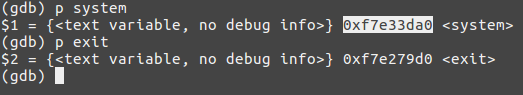
\epsfig{file=prob_2_part_1.png, height=2in, width=7in}
	\caption{Address of System and Exit calls.}
\end{figure}

\begin{figure}
	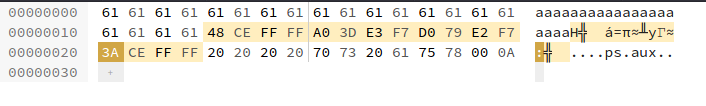
\epsfig{file=prob_2_part_4.png, height=2in, width=7in}
	\caption{Edited binary file to be used in program execution.}
\end{figure}

\begin{figure}
	\centering
	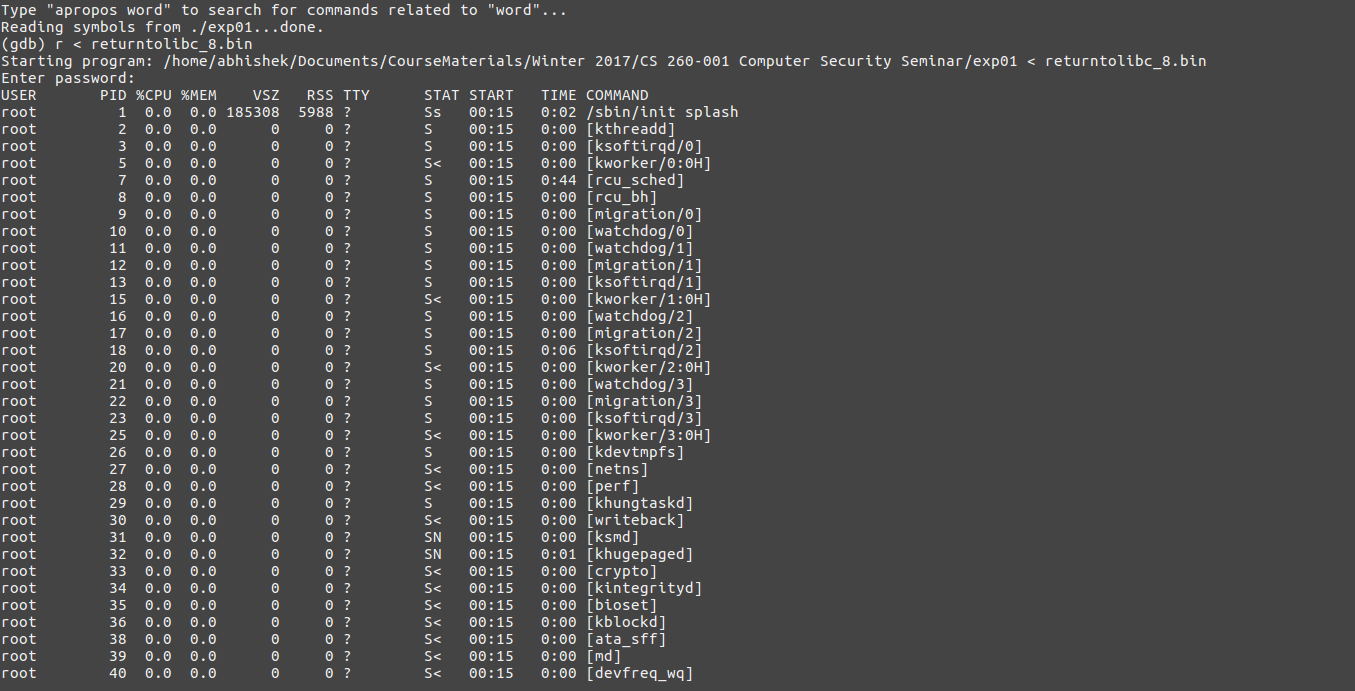
\epsfig{file=screen_1.png, height=4in, width=7in}
	\caption{Output of buffer overflow exploit.}
\end{figure}

\begin{figure}
	\centering
	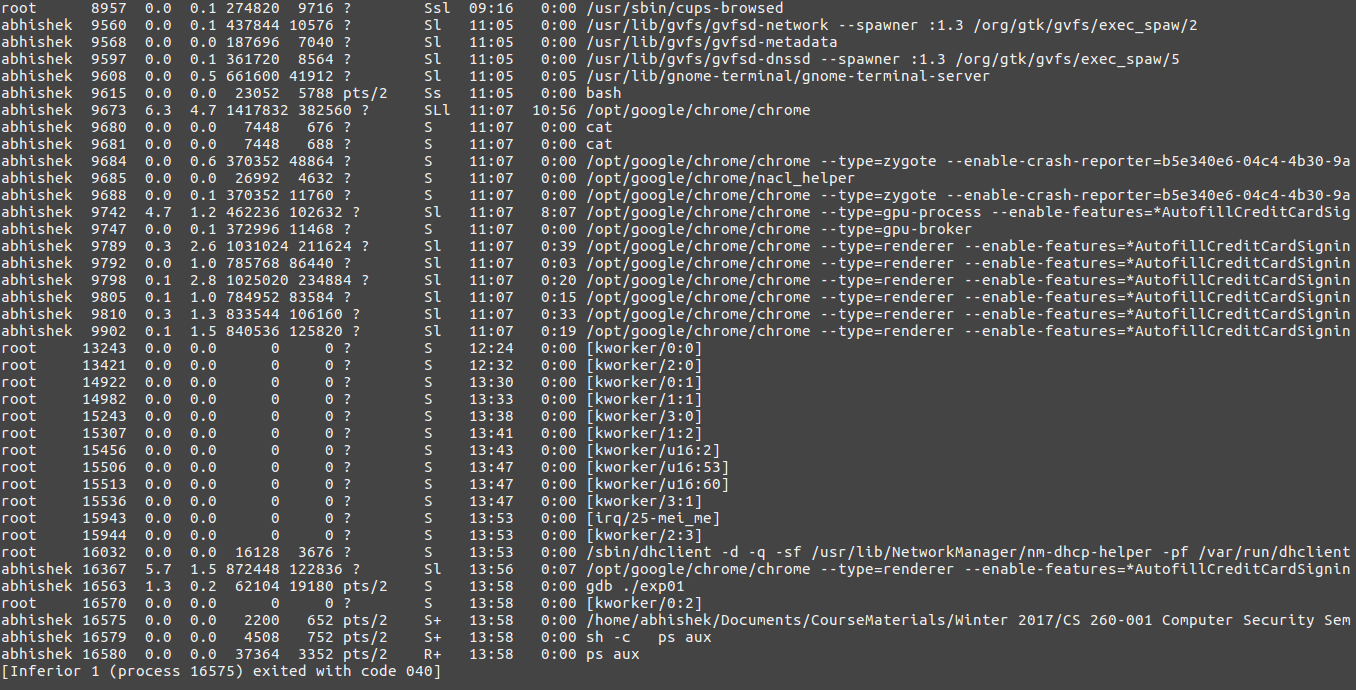
\epsfig{file=screen_2.png, height=4in, width=7in}
	\caption{Output of buffer overflow exploit.}
\end{figure}

\end{document}
